\documentclass[11pt,a4paper]{article}

\usepackage[margin=1in]{geometry}
\usepackage{graphicx}
\usepackage{booktabs}
\usepackage{hyperref}
\usepackage{natbib}
\usepackage[expansion=false]{microtype}
\usepackage{xcolor}
\usepackage{caption}
\usepackage{subcaption}
\usepackage{float}
\usepackage{enumitem}
\usepackage{tabularx}
\usepackage{amsmath}
\usepackage{array}

\hypersetup{
  colorlinks=true,
  linkcolor=black,
  citecolor=black,
  urlcolor=blue!50!black
}

\graphicspath{{figures/}{figures/gallery/}{figures/crops/}{figures/companion/}{figures/companion_gallery/}}
\captionsetup{font=small,labelfont=bf}
\setlength{\parskip}{0.35em}
\setlength{\parindent}{0pt}
\newcolumntype{L}[1]{>{\raggedright\arraybackslash}p{#1}}

\title{Evaluating and Adapting Small Vision-Language Models\\for Document Understanding}
\author{Ali Rasekh}
\date{}

\begin{document}
\maketitle

\begin{abstract}
We evaluate three small open vision-language models (VLMs) on a frozen DocVQA~\citep{mathew2021docvqa} design with development-selected InternVL3-1B~\citep{zhu2025internvl3,opengvlab2025internvl3_1b_card}, then compare a bounded language-attention LoRA~\citep{hu2022lora} adaptation under a sealed holdout.
Inference uses a custom PyTorch runner inspired by VLMEvalKit~\citep{duan2024vlmevalkit} DocVQA conventions, not a full VLMEvalKit benchmark execution.
On development primary ANLS, pretrained InternVL3-1B outperforms SmolVLM-256M/500M~\citep{marafioti2025smolvlm} and is selected as the deployment candidate (step~0).
Corrected LoRA v2 (update~200) is the fixed adaptation comparison.
On holdout ($n{=}504$), base ANLS is approximately $0.7927$ versus adapted $0.7993$ (paired $\Delta{=}{+}0.006639$).
A UCSF-cluster bootstrap 95\% interval of approximately $[{-}0.00530,{+}0.01905]$ includes zero: under this analysis, no clear improvement is established, and we make no equivalence claim.
Post-holdout supplementary Pascal development analyses (Appendix~\ref{app:pascal}) further probe visual-tile budgets, three-seed LoRA variability, and dependence on the correct document image; they do not change the sealed selection or official holdout result.
\end{abstract}

\section{Introduction and research questions}

Document visual question answering requires reading text, layout, and tables from page images~\citep{mathew2021docvqa}.
Small open VLMs enable reproducible cluster experiments, but published numbers often mix evaluation kits, preprocessing budgets, and metric variants.
This report answers four questions under a frozen protocol:
\begin{enumerate}[leftmargin=1.2em,itemsep=0.15em]
  \item How do three pretrained configured systems compare on a fixed DocVQA development split under a shared primary metric?
  \item Does bounded language-attention LoRA of the selected InternVL system improve development primary ANLS enough to replace step~0?
  \item On a once-evaluated holdout, how do the four systems score?
  \item Does a paired UCSF-cluster bootstrap support a clear adapted-minus-base gain?
\end{enumerate}
Comparisons are \emph{configured-system} comparisons (weights, native preprocess, decoding, prompts), not isolated architecture effects.

\paragraph{Model selection (eligibility, not a survey).}
We restricted candidates to small open instruct VLMs compatible with our pinned PyTorch/Transformers stack and a roughly sub-billion-parameter operating budget.
SmolVLM-256M and SmolVLM-500M~\citep{marafioti2025smolvlm} provide two sizes within one Idefics3-style family with documented efficient multimodal recipes.
InternVL3-1B~\citep{zhu2025internvl3,opengvlab2025internvl3_1b_card} adds a distinct InternVL family with an official dynamic document-oriented visual preprocess.
Together they cover family diversity and documented document/OCR-relevant capability without an exhaustive model survey.

\paragraph{From development observations to a bounded adaptation hypothesis.}
On development runs we observed recurring error modes: field/table-cell selection mistakes (wrong column or nearby cell), entity/text confusions among co-occurring names or phrases, and answer-format sensitivity (especially trailing punctuation for SmolVLM).
These observations motivate a \emph{hypothesis}, not a guarantee: language-attention LoRA may adjust task-conditioned answer selection and short-phrase formatting while leaving vision features fixed.
Freezing the vision backbone and connector deliberately limits the method's ability to fix visual-detail or extraction failures that require better visual encoding.
Under our compute budget, adapting only language attention on a 2000-example subset for 200 updates was practical and informative: it tests whether a cheap, localized adaptation moves primary development ANLS enough to displace the pretrained baseline.

\section{Task, data roles, and metrics}

\paragraph{Why DocVQA.}
DocVQA provides short extractive answers over real document pages with multi-reference answers~\citep{mathew2021docvqa}.

\paragraph{One dataset, several roles.}
All subsets come from HuggingFaceM4/DocumentVQA revision \texttt{a44195f8\ldots} (validation for smoke/dev/holdout; train shard for the adaptation subset).
Table~\ref{tab:data} lists roles; counts were verified against frozen manifests.
This is \textbf{not} a collection of independent benchmarks.

\begin{table}[H]
\centering
\caption{DocVQA roles used in this project (manifest-verified).}
\label{tab:data}
\begin{tabular}{@{}lrrp{5.2cm}@{}}
\toprule
Role & Questions & UCSF groups & Notes \\
\midrule
Smoke & 8 & 7 & Pipeline check \\
Development & 208 & 45 & Selection / comparison \\
Train (prepared) & 2000 & 298 & Adaptation pool; 1600 unique examples seen \\
Robustness (dev) & 54 & 16 & Synthetic stress subset of development \\
Holdout v2 & 504 & 109 & Sealed final evaluation \\
\bottomrule
\end{tabular}
\end{table}

\paragraph{Split construction (accurate history).}
Initial frozen splits were sampled with \texttt{doc\_id} grouping.
A later source-group audit found UCSF-level overlap between development and holdout~v1.
\textbf{Development membership was retained} after that audit; \textbf{holdout was rebuilt} as holdout\_v2 to remove UCSF overlap with smoke/development~\citep{mathew2021docvqa}.
We do not claim both splits were originally sampled under the corrected UCSF grouping scheme.
Image integrity (PNG hashes) was audited for the frozen sets.

\paragraph{Relation to VLMEvalKit.}
VLMEvalKit~\citep{duan2024vlmevalkit} documents a DocVQA\_VAL route and ANLS-style utilities.
Our evaluation is a custom greedy runner with frozen manifests and a project primary metric.
We do \textbf{not} claim a full VLMEvalKit leaderboard run.
Secondary diagnostics (VLMEvalKit-compatible ANLS; strip $\le$1 trailing period after normalize) are not used for selection.

\paragraph{Primary metric (self-contained).}
Primary score is project metric \texttt{anls\_normalized\_strict\_v2} (normalized strict ANLS), \textbf{not} claimed byte-identical to official Pix2Struct~\citep{lee2023pix2struct} or VLMEvalKit scorers.
Normalization: lowercase, strip ends, collapse internal whitespace to single spaces.
Let $\mathrm{NL}$ be Levenshtein distance divided by $\max(|\hat{y}|,|y|)$ on the normalized prediction and reference strings.
Per-reference score is $1-\mathrm{NL}$ if $\mathrm{NL}<0.5$, else $0$.
Example score is the maximum over valid nonempty references.
Primary EM uses the same normalization and requires equality to some reference (no punctuation stripping).
Failures and missing predictions count as zero in requested-set means over the full question set.

\section{Systems and visual preprocessing}

\begin{table}[H]
\centering
\caption{Pretrained configured systems. Parameter counts are measured unique parameters.}
\label{tab:systems}
\begin{tabular}{@{}lrl@{}}
\toprule
System & Unique params & Notes \\
\midrule
SmolVLM-256M-Instruct & 256{,}484{,}928 & Idefics3-style \\
SmolVLM-500M-Instruct & 507{,}482{,}304 & Idefics3-style \\
InternVL3-1B & 938{,}193{,}024 & Dynamic 448px tiles \\
\bottomrule
\end{tabular}
\end{table}

Native visual preprocessing differs across families and yields unequal visual-token budgets.
SmolVLM uses processor defaults; InternVL3-1B uses the official dynamic preprocess (448px tiles, \texttt{max\_num}${}={}$12, thumbnail enabled) from the model card~\citep{opengvlab2025internvl3_1b_card}.

\paragraph{InternVL3-1B backbone names.}
The official InternVL3-1B model card~\citep{opengvlab2025internvl3_1b_card} identifies vision backbone \texttt{InternViT-300M-448px-V2\_5} and language backbone \texttt{Qwen2.5-0.5B}.
Runtime Transformers architecture notes report class \texttt{Qwen2ForCausalLM}; that class name is an implementation detail, not a reason to name the backbone simply ``Qwen2''.
Vision runtime module is InternVisionModel within InternVLChatModel; connector uses downsample ratio $0.5$ (pixel-unshuffle style).

\section{Model profiles, qualitative gaps, and measurement plan}
\label{sec:profiles}

\paragraph{Model profiles (documented sources).}
SmolVLM-256M/500M~\citep{marafioti2025smolvlm} are compact Idefics3-style instruct VLMs.
The public Hugging Face model card for SmolVLM-256M-Instruct states that training data come from \textbf{The Cauldron} and \textbf{Docmatix}, with emphasis on document understanding (${\approx}25\%$) and image captioning (${\approx}18\%$), plus broader multimodal instruction mixtures; a full exhaustive dump of mixture members is not provided on the card.
InternVL3-1B~\citep{zhu2025internvl3,opengvlab2025internvl3_1b_card} pairs \texttt{InternViT-300M-448px-V2\_5} with a \texttt{Qwen2.5-0.5B}-initialized language component and documents \textbf{Native Multimodal Pre-Training} that interleaves multimodal sequences with large-scale text corpora (card/paper-level description).
The InternVL3 card does \textbf{not} publish a complete dataset inventory sufficient to prove or disprove DocVQA contamination.
We therefore report the disclosed mixtures/methods above and still treat residual pretrained exposure as an open risk (Limitations), not a settled fact.

\paragraph{Qualitative knowledge-gap sample (development; descriptive only).}
From InternVL3-1B development predictions we drew a seeded sample of $n{=}20$ non-perfect examples (48 non-perfect among 208; selection rule in \texttt{results/internvl\_error\_sample\_v1.json}).
This sample is \textbf{qualitative and not a quantitative error taxonomy} for the full split.
Recurring observed tags in the inspected sample include text/checkbox reading mistakes, nearby field or table-cell confusions, and formatting/entity mismatches between prediction and references.
These observations motivated the \emph{working} hypothesis that language-attention LoRA might help short-phrase formatting and answer selection while leaving vision features fixed---a post-hoc interpretation of development errors, \textbf{not} a pre-registered experimental hypothesis.

\paragraph{Expected outcomes and measurement criteria (stated retrospectively).}
Under the frozen protocol we expected: (i)~InternVL to lead SmolVLM on development primary ANLS given its stronger document preprocess; (ii)~bounded LoRA either to improve development ANLS enough to displace step~0 or to show only small movements; (iii)~holdout to report absolute configured-system scores with a paired InternVL adapted$-$base interval that may include zero.
Measurement criteria remained primary \texttt{anls\_normalized\_strict\_v2} on frozen requested sets, with EM secondary and formatting diagnostics non-selective.
Improvement plan if revisiting adaptation: larger multi-seed budgets, matched visual-token settings across families, and diagnostics that isolate visual grounding beyond whole-page replacement (Appendix~\ref{app:pascal}).

\paragraph{Software stack and edge extrapolation.}
The tested stack is PyTorch $2.5.1{+}$cu118 with Transformers $4.48.3$ and PEFT $0.14.0$ on server GPUs (Neumann A100 / Pascal V100 allocations as recorded per experiment).
Latency and peak-memory figures characterize those server allocations only; they do \textbf{not} transfer to edge or mobile devices without re-measurement under the target runtime.
Generic CPU-only \texttt{pip install} environments are insufficient to reproduce GPU timings or bf16 training behavior.

\section{Development comparison and selection}

\begin{table}[H]
\centering
\caption{Development primary metrics ($n{=}208$). Diagnostic EM strips $\le$1 trailing period after normalize (secondary).}
\label{tab:dev}
\begin{tabular}{@{}lrrr@{}}
\toprule
System & ANLS & EM & Diag.\ EM \\
\midrule
SmolVLM-256M & 0.5568 & 0.2596 & 0.4952 \\
SmolVLM-500M & 0.6095 & 0.0433 & 0.6298 \\
InternVL3-1B (step 0) & 0.8324 & 0.7692 & 0.7692 \\
\bottomrule
\end{tabular}
\end{table}

Table~\ref{tab:dev} summarizes pretrained development scores on Neumann (InternVL base ANLS $0.8324$).
Pascal supplementary matched-base ANLS $0.8276$ is a separate recorded run; see \S\ref{sec:pascal}.
Under the pre-declared rule (primary development ANLS; earlier step on ties), InternVL step~0 is the deployment candidate.
Corrected LoRA v2 scored ${\approx}0.8263$ (update~100) and ${\approx}0.8290$ (update~200), both below step~0.
Best corrected trained checkpoint is update~200 (adaptation comparison only).
\textbf{Selection protocol:} freeze deployment = step~0 and adaptation comparison = LoRA v2 u200 from development; holdout rankings are reported but do not change that selection.

\section{Adaptation recipe}

\begin{figure}[H]
\centering
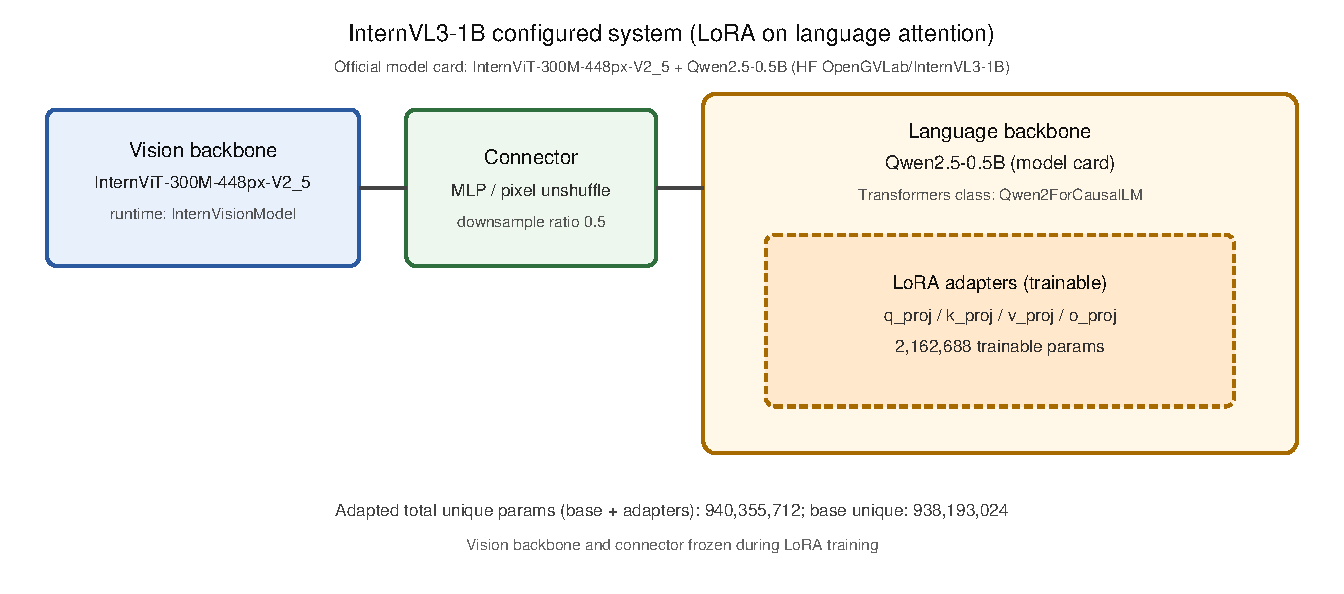
\includegraphics[width=0.95\linewidth]{architecture_lora_placement.pdf}
\caption{InternVL3-1B with LoRA on language-model attention. Backbone names follow the official model card~\citep{opengvlab2025internvl3_1b_card}.}
\label{fig:arch}
\end{figure}

\begin{figure}[H]
\centering
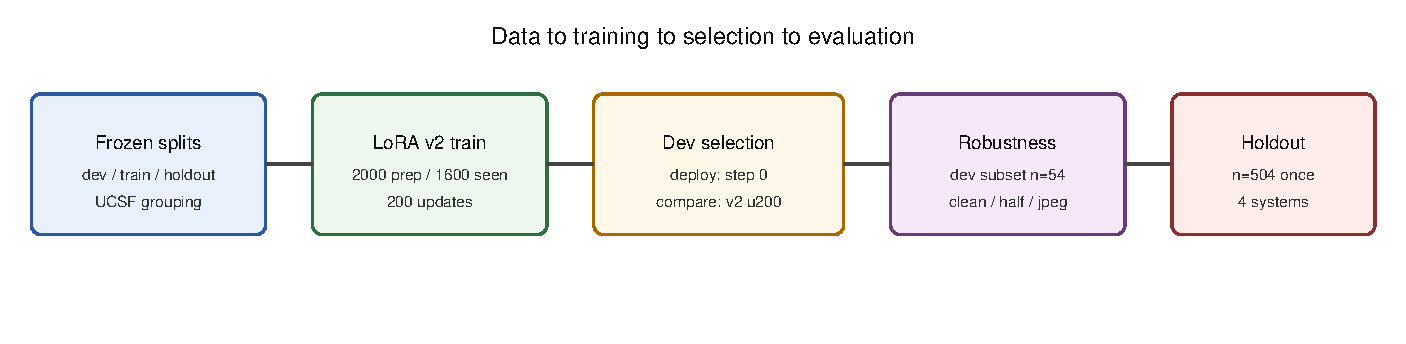
\includegraphics[width=0.98\linewidth]{pipeline_flow.pdf}
\caption{Data preparation $\rightarrow$ LoRA training $\rightarrow$ development selection $\rightarrow$ robustness subset $\rightarrow$ sealed holdout.}
\label{fig:pipeline}
\end{figure}

LoRA~\citep{hu2022lora} targets \texttt{language\_model} attention \texttt{q\_proj}/\texttt{k\_proj}/\texttt{v\_proj}/\texttt{o\_proj} ($r{=}16$, $\alpha{=}32$, dropout $0.05$), freezing vision and connector.
Adapted total unique parameters including adapters: $940{,}355{,}712$; trainable: $2{,}162{,}688$.

\paragraph{Supervised labels (corrected v2).}
Historical v1 training duplicated the assistant end-of-turn token (2000/2000 audited examples).
v1 is historical/superseded; we do not claim it caused every score difference, and we do not compare v1/v2 loss magnitudes as the same objective.
Corrected v2 uses a single assistant EOS; labels supervise the assistant answer span only (prompt tokens masked).

\paragraph{Bounded training (actual config).}
Target answer = first nonempty source-listed answer.
Optimizer AdamW (lr $5{\times}10^{-5}$, weight decay $0.01$); linear warmup schedule over 10 updates then decay across 200 updates; grad clip $1.0$; microbatch 1; grad accum 8; bf16 when supported; seed 42; max sequence length 8192.
From the prepared 2000-example subset, training presented 1600 sample presentations (1600 unique QIDs under shuffle+wrap).
Figure~\ref{fig:loss}: first-20 mean ${\approx}0.2561$, last-20 mean ${\approx}0.2143$ (full precision retained in artifacts).

\begin{figure}[H]
\centering
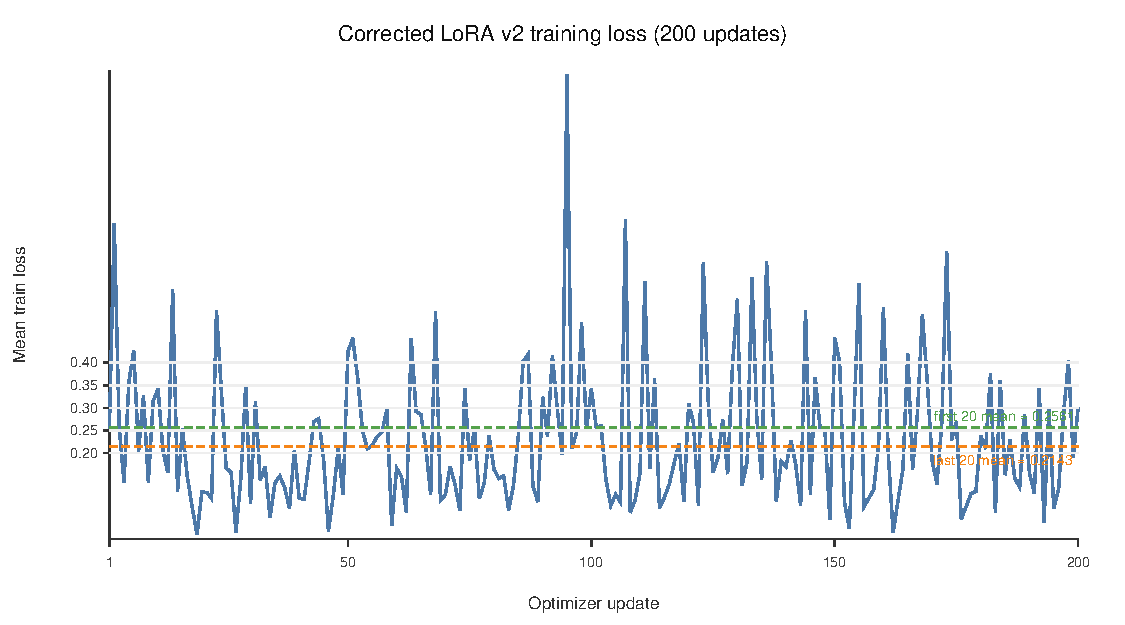
\includegraphics[width=0.90\linewidth]{train_loss_v2.pdf}
\caption{Corrected LoRA v2 per-update training loss with numeric axis ticks.}
\label{fig:loss}
\end{figure}

\section{Development robustness (limited)}

On a fixed development subset ($n{=}54$ / 16 UCSF groups) we apply three image conditions before native preprocess:
\emph{clean}; \emph{half-detail} (BICUBIC downsample by floor$(w/2)$, floor$(h/2)$, then restore exact original dimensions); \emph{JPEG q40} (quality 40, Pillow \texttt{subsampling=2} / 4:2:0).
Preserving dimensions keeps InternVL dynamic tile counts comparable across conditions so the stress is content degradation, not a different tiling budget.
Figure~\ref{fig:robust} shows small differences; this is not a corruption benchmark.
Phase~3B v1 robustness figures remain historical only.

\begin{figure}[H]
\centering
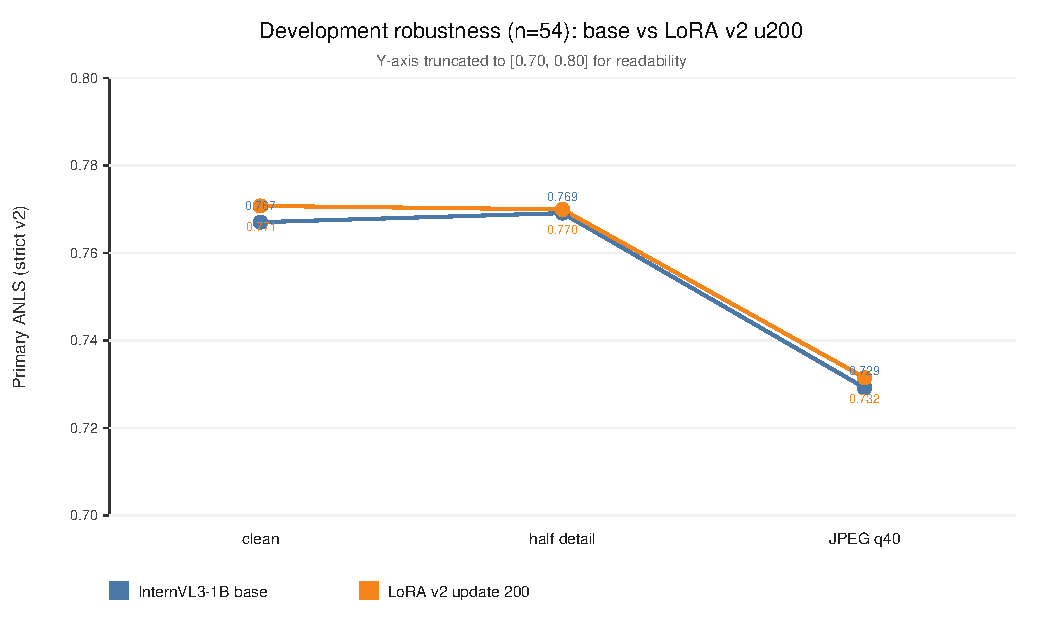
\includegraphics[width=0.90\linewidth]{robustness_v2_anls.pdf}
\caption{Development robustness primary ANLS (dot/line; y-axis truncated to $[0.70,0.80]$).}
\label{fig:robust}
\end{figure}

\section{Holdout results}

Protocol freeze revision \texttt{a9b0695\ldots}; four systems once on holdout\_v2 ($n{=}504$; job 84636; A100-PCIE-40GB).
Latency is CUDA-synchronized \emph{generation-only} time (warmup excluded), not end-to-end wall-clock.
Table~\ref{tab:holdout} and Figure~\ref{fig:holdout} report primary metrics; Appendix~\ref{app:latency} adds p95 latency and peak allocated memory.

\begin{table}[H]
\centering
\caption{Holdout primary metrics ($n{=}504$). Values are fractions in $[0,1]$.}
\label{tab:holdout}
\begin{tabular}{@{}lrrr@{}}
\toprule
System & ANLS & EM & Med.\ gen.\ (s) \\
\midrule
SmolVLM-256M & 0.5753 & 0.3234 & 0.214 \\
SmolVLM-500M & 0.5997 & 0.0694 & 0.244 \\
InternVL3-1B (base) & 0.7927 & 0.7282 & 0.482 \\
InternVL + LoRA v2 u200 & 0.7993 & 0.7401 & 0.538 \\
\bottomrule
\end{tabular}
\end{table}

\begin{figure}[H]
\centering
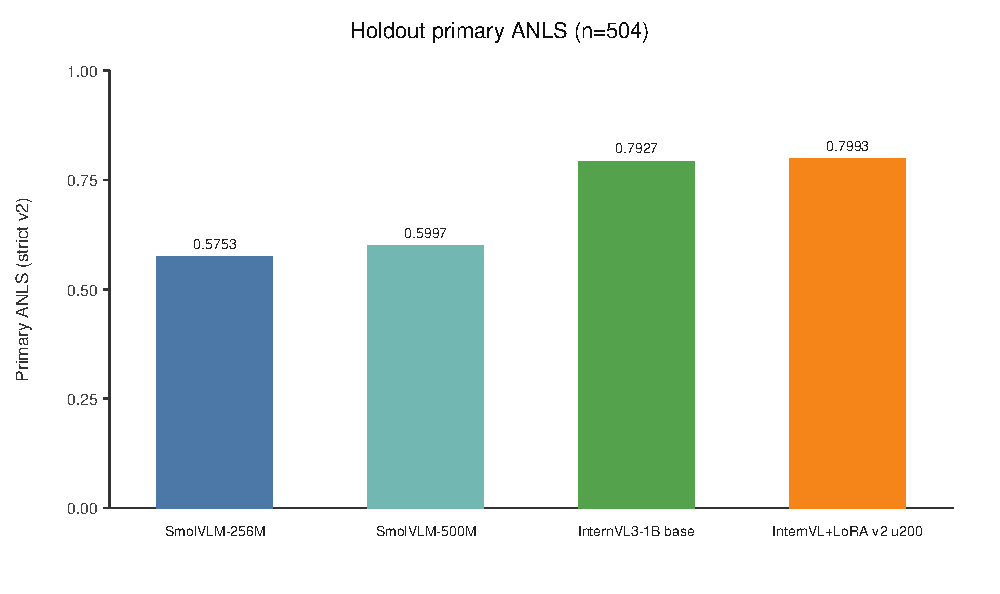
\includegraphics[width=0.88\linewidth]{holdout_primary_anls.pdf}
\caption{Holdout primary ANLS for the four configured systems.}
\label{fig:holdout}
\end{figure}

Secondary VLMEvalKit-style ANLS preserves the InternVL base/adapted ordering.
SmolVLM-500M shows formatting sensitivity: primary EM ${\approx}0.0694$ vs diagnostic EM ${\approx}0.6052$.

\paragraph{Paired adaptation analysis.}
Point estimate adapted$-$base ANLS ${=}{+}0.006639$ (about $+0.66$ percentage points if mapped to a 0--100 scale; we report fractions).
UCSF-cluster bootstrap ($B{=}2000$, seed 42) yields 95\% CI approximately $[{-}0.00530,{+}0.01905]$ (Figure~\ref{fig:ci}).
The interval includes zero: no clear improvement is established; we do not claim equivalence.

\begin{figure}[H]
\centering
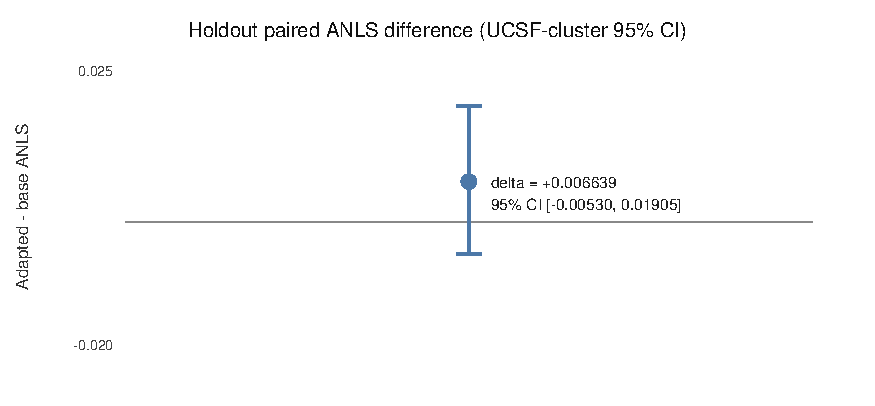
\includegraphics[width=0.78\linewidth]{paired_adaptation_ci.pdf}
\caption{Paired holdout ANLS difference with UCSF-cluster 95\% CI.}
\label{fig:ci}
\end{figure}

\section{Illustrative input/output examples}

Examples are deterministically selected (gallery manifest) and illustrative, not performance-representative.
Crops are marked; full-page context remains available under \texttt{data/images/docvqa\_holdout\_v2/}.

\paragraph{Shared table-column error (qid 307).}
Duration for ``Replace Flex Tester'' is 6 months; both systems predict \texttt{1.0} (PRIORITY cell).
Figure~\ref{fig:table} shows a labeled crop of the relevant rows.

\paragraph{Adaptation improvement (qid 18564).}
Invoice addressee question: base predicts ``Dr.\ Samuel Deadwyler'' (body/description name); adapted predicts ``Dr.\ J.\ H.\ Robinson'' (recipient box).
Figure~\ref{fig:improv} pairs a marked full page with the addressee crop.

\paragraph{Adaptation regression (qid 792).}
Letter mentioning a free sample of SAMSON: base answers ``SAMSON''; adapted answers ``free sample''.
Figure~\ref{fig:regr} pairs marked full page and sentence crop.

\begin{figure}[H]
\centering
\begin{subfigure}{0.48\linewidth}
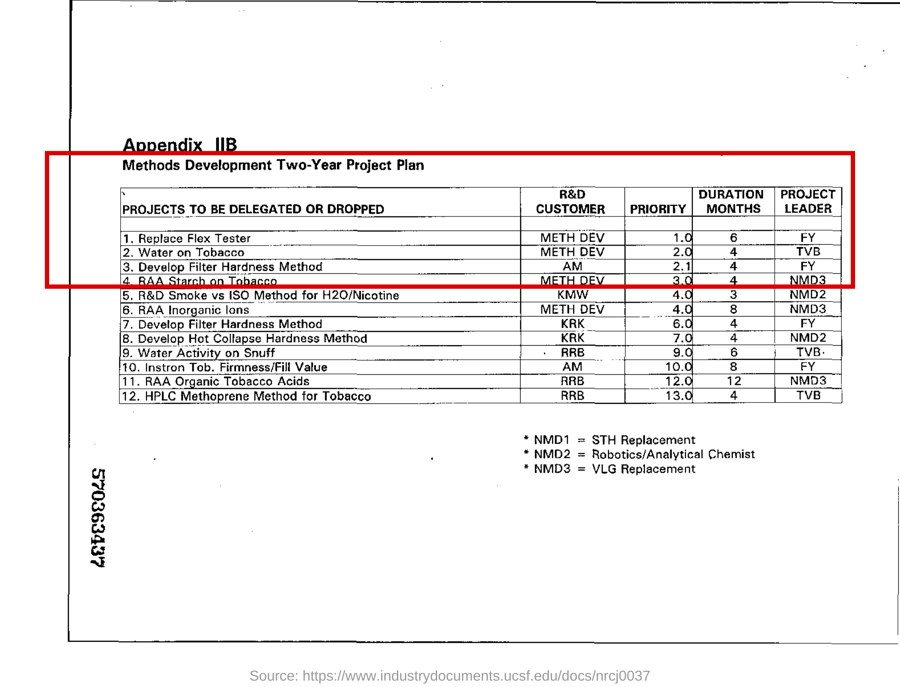
\includegraphics[width=\linewidth]{full_marked_table_qid_307.jpg}
\caption*{Full page (crop box marked)}
\end{subfigure}\hfill
\begin{subfigure}{0.48\linewidth}
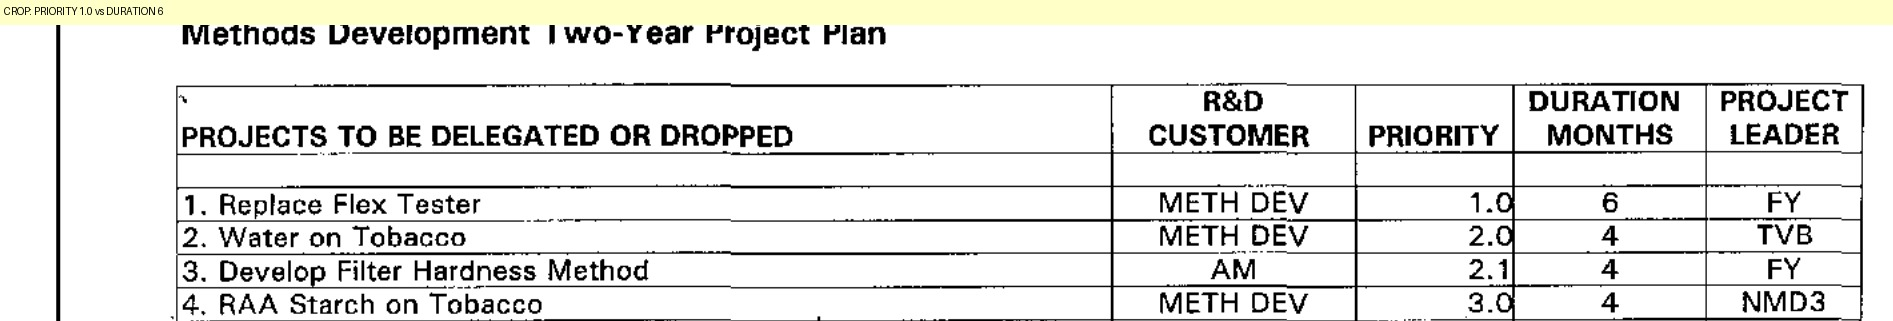
\includegraphics[width=\linewidth]{crop_table_column_error_qid_307.jpg}
\caption*{Evidence crop}
\end{subfigure}
\caption{Illustrative shared error (qid 307): PRIORITY vs DURATION.}
\label{fig:table}
\end{figure}

\begin{figure}[H]
\centering
\begin{subfigure}{0.48\linewidth}
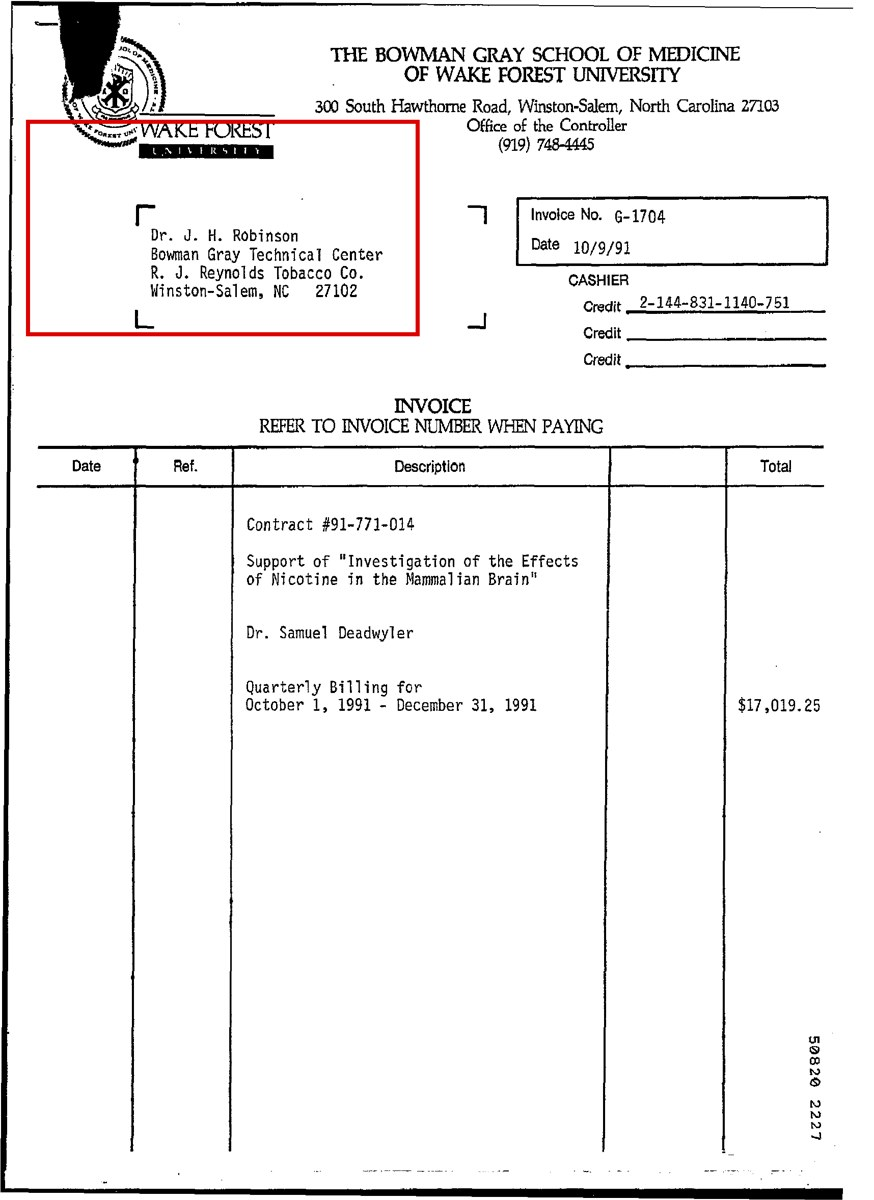
\includegraphics[width=\linewidth]{full_marked_improvement_qid_18564.jpg}
\caption*{Full page (crop box marked)}
\end{subfigure}\hfill
\begin{subfigure}{0.48\linewidth}
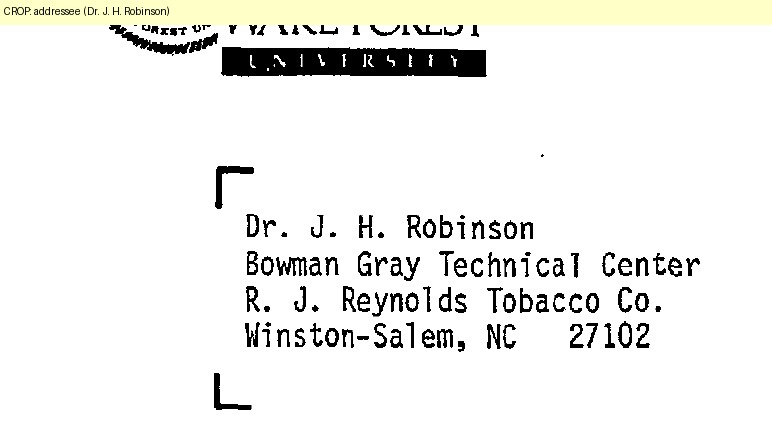
\includegraphics[width=\linewidth]{crop_improvement_addressee_qid_18564.jpg}
\caption*{Addressee crop}
\end{subfigure}
\caption{Illustrative adaptation improvement (qid 18564).}
\label{fig:improv}
\end{figure}

\begin{figure}[H]
\centering
\begin{subfigure}{0.48\linewidth}
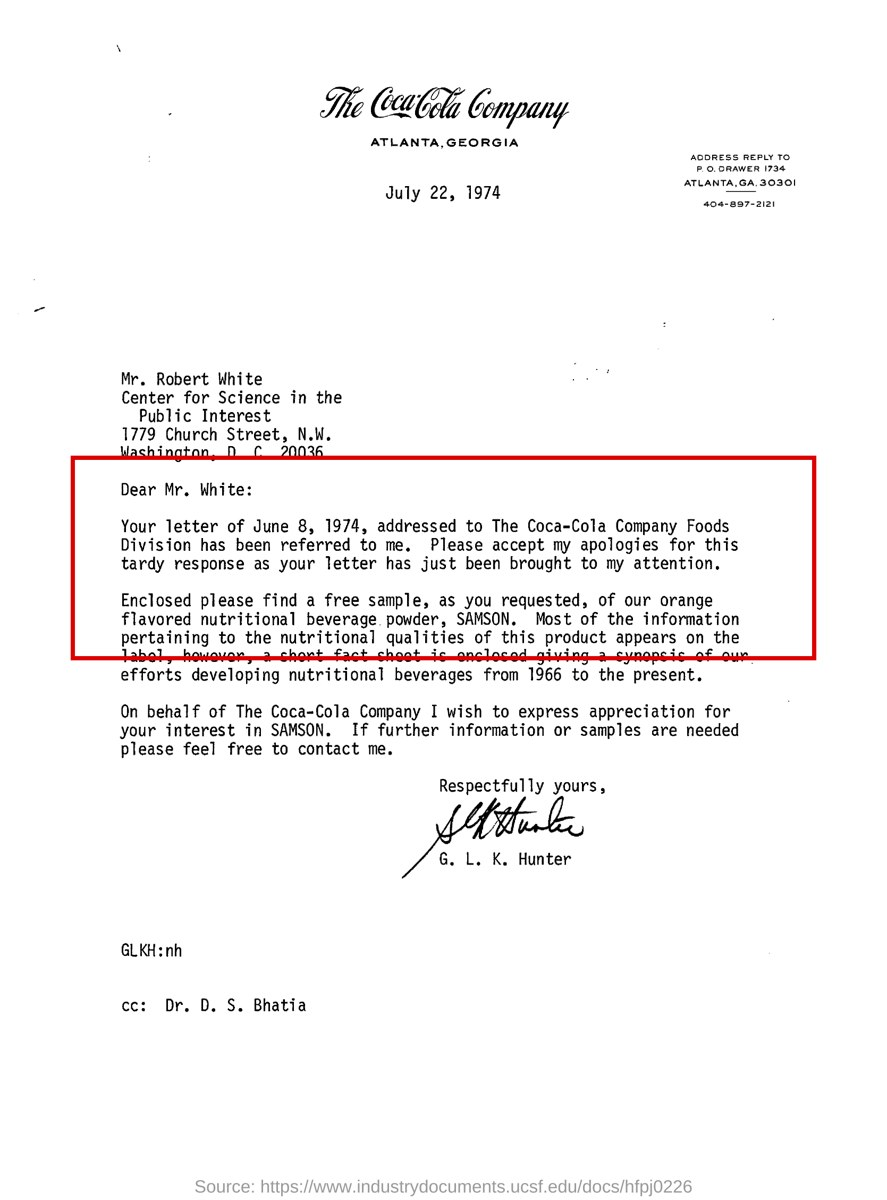
\includegraphics[width=\linewidth]{full_marked_regression_qid_792.jpg}
\caption*{Full page (crop box marked)}
\end{subfigure}\hfill
\begin{subfigure}{0.48\linewidth}
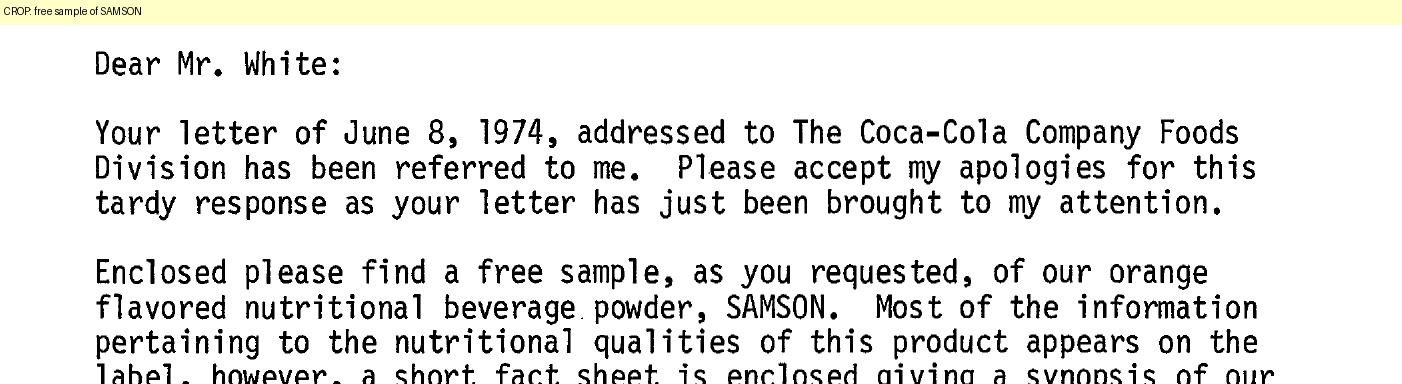
\includegraphics[width=\linewidth]{crop_regression_samson_qid_792.jpg}
\caption*{Sentence crop}
\end{subfigure}
\caption{Illustrative adaptation regression (qid 792).}
\label{fig:regr}
\end{figure}

\section{Limitations and future work}

\begin{itemize}[leftmargin=1.2em,itemsep=0.15em]
  \item Sampled DocVQA evaluation, not official full-benchmark leaderboard parity.
  \item Unequal native visual-token budgets across families.
  \item Possible pretrained exposure to DocVQA-related data is not ruled out from public cards alone.
  \item Original selection used a single seed and bounded LoRA budget; historical v1 double-EOT training superseded.
  \item Phase~3B robustness evidence is limited to the fixed synthetic development subset (clean / half-detail / JPEG~q40); it is distinct from the later visual-input-dependence study.
  \item Bootstrap CIs describe this holdout resampling design only; they are not seed SDs.
  \item Supplementary Pascal runs used V100 BF16 usability (not native CC$\ge$8) and, for P3, a documented cross-node GPU SKU change (Appendix~\ref{app:pascal}).
\end{itemize}

\section{Supplementary Pascal development analyses}
\label{sec:pascal}

After sealing holdout selection, we ran \emph{post-holdout} development analyses on Pascal under companion ownership (\texttt{companion/pascal/}).
They did \textbf{not} change the deployment candidate (InternVL step~0) or official holdout scores.
Details and figures are in Appendix~\ref{app:pascal}; compact evidence is under \texttt{companion/pascal/results/}.

\paragraph{Visual-budget ablation (P1).}
On the frozen InternVL3-1B \textbf{base} (no LoRA), reducing only \texttt{max\_num} from 12$\to$4$\to$1 on development ($n{=}208$) lowers primary ANLS from approximately $0.8276$ to $0.7588$ to $0.5595$, with corresponding reductions in actual tile usage and request latency on the recorded V100 run.
This is a within-runtime quality/cost trade-off under matched decoding, not a claim about other GPUs.
The Pascal matched-base figure $0.8276$ is a \emph{separate recorded run} from the earlier Neumann development InternVL base score $0.8324$ in Table~\ref{tab:dev}; documented differences include host/GPU (Pascal V100 vs Neumann A100), allocation, and job identity.
We do \textbf{not} assert a single verified cause for that score gap; Pascal tables use the Pascal matched control only.

\paragraph{Three-seed fixed-budget LoRA (P3).}
Repeating corrected v2 settings for seeds $\{42,43,44\}$ to update~200 yields development ANLS $\{0.8193,0.8178,0.8317\}$ versus a matched fresh base $0.8276$.
Arithmetic mean $0.8229$; \textbf{sample SD across three seeds} $0.0076$ (ddof${=}1$; \emph{not} a confidence interval).
Two seeds fall below base and one is slightly above: under this fixed configuration and budget we observe \textbf{no consistent improvement} over the matched base.
This does \textbf{not} claim that LoRA generally fails.
Each completed run saw 1600 unique QIDs from the 2000-example pool (80\% coverage); sample order/membership differs by seed.
These Pascal adapters are separate from the official Neumann v2 u200 adaptation comparison.

\paragraph{Visual-input dependence.}
On the pinned InternVL3-1B base only, replacing the correct page with a white or unrelated development image reduced development ANLS by approximately \textbf{78 percentage points}, indicating strong dependence on the correct visual input.
That summary is not an exact decomposition of performance, not proof of fine-grained grounding, and not evidence for or against contamination.
White residual ANLS ${\approx}0.042$; unrelated ${\approx}0.047$ (scored against the \emph{original} question references).
Prediction agreement with the clean prediction is a separate diagnostic from correctness; agreement uses only pairs where both records succeed.

\section{Conclusion}

Under the frozen protocol, InternVL3-1B step~0 remains the development-selected deployment candidate; corrected LoRA v2 update~200 is the fixed adaptation comparison.
Holdout shows a small positive ANLS point estimate whose UCSF-cluster 95\% CI includes zero.
Configured-system gaps between SmolVLM and InternVL are large; adaptation gains under the original budget are not clearly established.
Supplementary Pascal analyses reinforce a strong visual-input dependence for the selected base and show no consistent three-seed LoRA gain under the fixed corrected recipe, without revising sealed selection.

\appendix
\section{Reproducibility pins}
\label{app:repro}

{\small
\begin{tabularx}{\linewidth}{@{}L{3.2cm}X@{}}
\toprule
Item & Pin \\
\midrule
Python / torch / transformers / peft & 3.11 / 2.5.1{+}cu118 / 4.48.3 / 0.14.0 \\
SmolVLM-256M & \texttt{HuggingFaceTB/SmolVLM-256M-Instruct} @ \texttt{7e3e67ed\ldots} \\
SmolVLM-500M & \texttt{HuggingFaceTB/SmolVLM-500M-Instruct} @ \texttt{a7da5b98\ldots} \\
InternVL3-1B & \texttt{OpenGVLab/InternVL3-1B} @ \texttt{4415a3b8\ldots} \\
Vision / language (card) & \texttt{InternViT-300M-448px-V2\_5} / \texttt{Qwen2.5-0.5B} \\
DocVQA HF mirror & \texttt{HuggingFaceM4/DocumentVQA} @ \texttt{a44195f8\ldots} \\
VLMEvalKit reference rev & \texttt{54a063c5\ldots} (route/metric reference only) \\
Eval protocol freeze & git \texttt{a9b0695\ldots} \\
LoRA v2 u200 adapter SHA256 & \texttt{3c2c34cd\ldots c344180a} \\
Holdout job & 84636 \\
\bottomrule
\end{tabularx}
}

Commands: \texttt{reports/README.md}, \texttt{docs/report/SUBMISSION\_GUIDE.md}.
Official LoRA v2 u200 adapter weights are tracked under \texttt{artifacts/internvl3\_1b\_lora\_v2\_u200/} (SHA256 in \texttt{artifacts/internvl3\_1b\_lora\_v2\_u200\_adapter\_sha256.txt}); base weights and DocVQA images must still be downloaded separately.

\section{Holdout latency and memory}
\label{app:latency}

\begin{table}[H]
\centering
\caption{Generation-only latency and peak allocated GPU memory (holdout; from frozen summaries).}
\label{tab:latency}
\begin{tabular}{@{}lrrr@{}}
\toprule
System & Med.\ (s) & p95 (s) & Peak alloc.\ (GiB) \\
\midrule
SmolVLM-256M & 0.214 & 0.410 & 2.78 \\
SmolVLM-500M & 0.244 & 0.427 & 3.26 \\
InternVL3-1B (base) & 0.482 & 0.647 & 3.42 \\
InternVL + LoRA v2 u200 & 0.538 & 0.799 & 3.43 \\
\bottomrule
\end{tabular}
\end{table}

\section{Historical v1 note}
v1 LoRA used duplicated supervised EOT labels; superseded by v2.
Do not compare v1/v2 losses as the same objective.
Chronology: \texttt{docs/progress/phase03c.md}.

\section{Supplementary Pascal evidence}
\label{app:pascal}

All tables below use the development requested set ($n{=}208$) unless noted.
Failures/missing count as zero; generation-cap hits remain in requested-set means.
These analyses are labeled \textbf{post-holdout supplementary development} work.

\subsection*{A. Visual-budget ablation (P1)}
Pinned InternVL3-1B base; conditions \texttt{max\_num}${}\in\{12,4,1\}$; greedy; \texttt{max\_new\_tokens}${}={}$64; Pascal V100 (BF16 usability).
Job 117225.

\begin{table}[H]
\centering
\caption{P1 development primary metrics by tile-budget cap (requested-set means).}
\label{tab:p1}
\begin{tabular}{@{}rrrr@{}}
\toprule
\texttt{max\_num} & ANLS & EM & Mean tiles (observed) \\
\midrule
12 & 0.8276 & 0.7644 & 12.58 \\
4 & 0.7588 & 0.6538 & 4.62 \\
1 & 0.5595 & 0.4183 & 1.00 \\
\bottomrule
\end{tabular}
\end{table}

\begin{figure}[H]
\centering
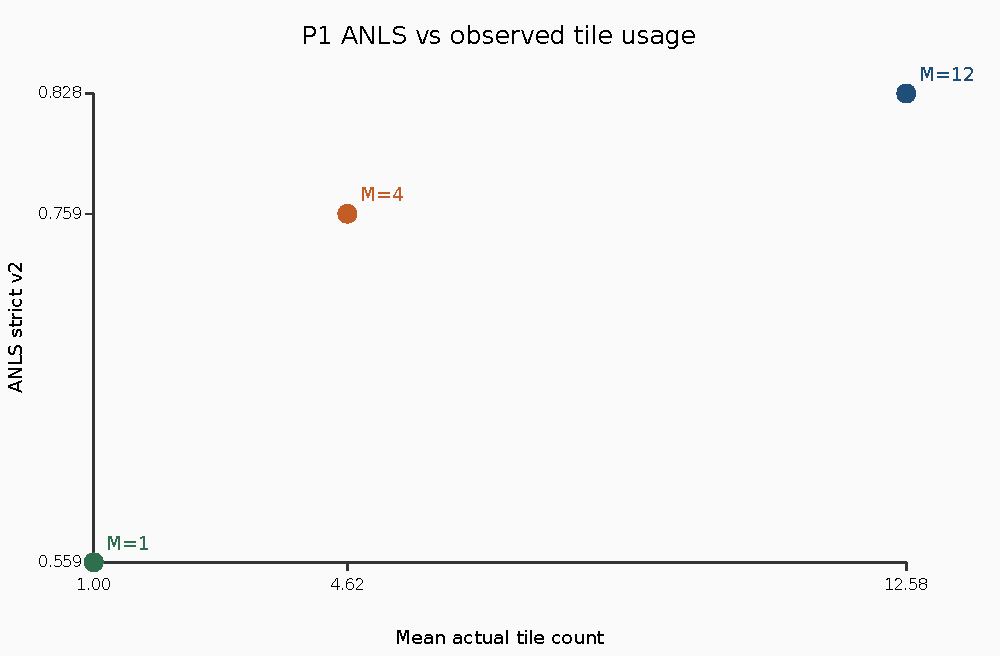
\includegraphics[width=0.72\linewidth]{p1_anls_vs_tile_usage.pdf}
\caption{P1: development ANLS versus observed mean tile usage under \texttt{max\_num} caps (InternVL3-1B base).}
\label{fig:p1}
\end{figure}

\subsection*{B. Three-seed corrected LoRA (P3)}
Settings match corrected v2 (seeds 42/43/44; 200 updates; accum~8).
Fresh-base and adapter evaluations share the development manifest denominator.
Figure~\ref{fig:p3anls} marks the common fresh base; Figure~\ref{fig:p3loss} shows raw loss (faint) with trailing 20-update means (samples may differ by seed).

\begin{table}[H]
\centering
\caption{P3 development ANLS/EM (requested set). Sample SD is across three seed ANLS values (ddof${=}1$), not a CI.}
\label{tab:p3}
\begin{tabular}{@{}rrrrr@{}}
\toprule
System & ANLS & EM & $\Delta$ANLS vs base & $\uparrow$/$\downarrow$/$=$ \\
\midrule
Fresh base & 0.8276 & 0.7644 & --- & --- \\
Seed 42 & 0.8193 & 0.7644 & $-0.0084$ & 5/6/197 \\
Seed 43 & 0.8178 & 0.7596 & $-0.0098$ & 8/7/193 \\
Seed 44 & 0.8317 & 0.7740 & $+0.0040$ & 6/3/199 \\
\midrule
3-seed mean / sample SD & 0.8229 & --- & --- & SD $0.0076$ \\
\bottomrule
\end{tabular}
\end{table}

\begin{figure}[H]
\centering
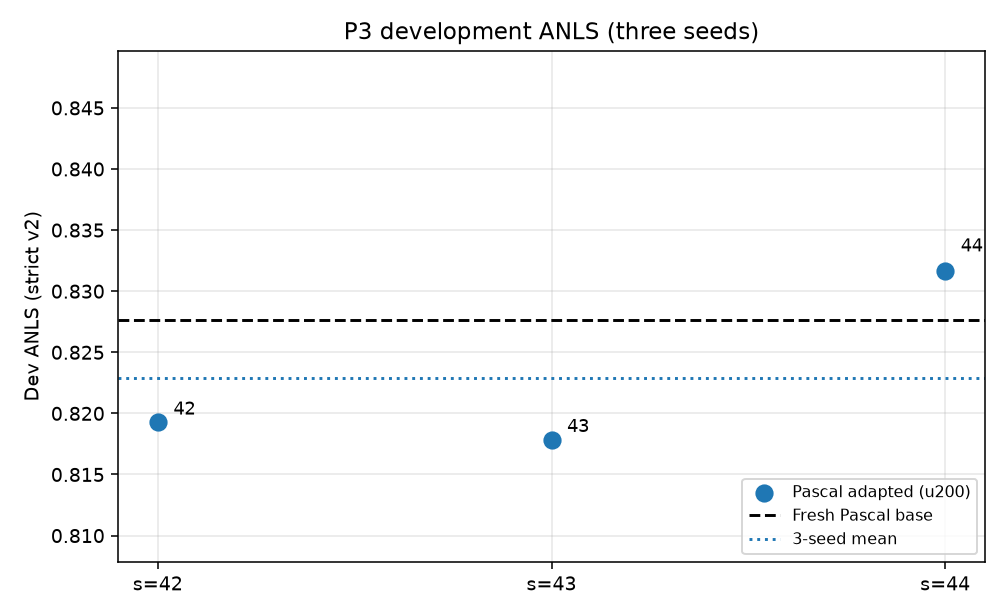
\includegraphics[width=0.78\linewidth]{p3_dev_anls.png}
\caption{P3 development ANLS for three Pascal seeds versus fresh base (dashed) and three-seed mean (dotted).}
\label{fig:p3anls}
\end{figure}

\begin{figure}[H]
\centering
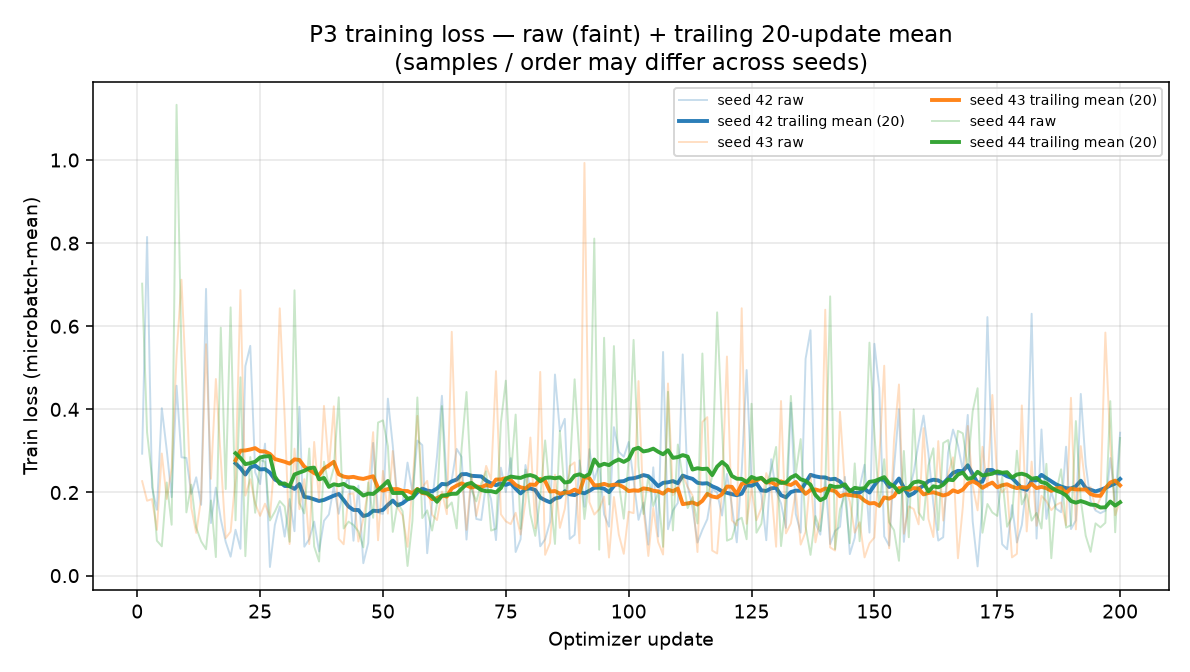
\includegraphics[width=0.92\linewidth]{p3_loss_curves.png}
\caption{P3 training loss: low-opacity raw traces and trailing 20-update means. Training examples can differ across seeds.}
\label{fig:p3loss}
\end{figure}

\paragraph{Coverage and provenance.}
Each completed run: 200 optimizer updates, 1600 presentations, 1600 unique QIDs (80\% of the 2000-pool).
Protocol deviation: seeds 42/43 trained on pascal-node10 (V100-SXM3); completed seed~44 and all four evaluations on pascal-node09 (V100-PCIE).
Interrupted 164-update seed~44 attempt preserved and excluded.
Official Neumann v2 u200 remains a separate historical reference.

\subsection*{C. Visual-input dependence}
Pinned InternVL3-1B \textbf{base} only (not a P3 adapter); conditions clean / white (exact original $W{\times}H$) / unrelated donor from the same 208-set.
Job 117260; one allocation.

\begin{table}[H]
\centering
\caption{Visual-input dependence on development ($n{=}208$ ok / 0 fail / 0 miss). Agreement denominator: pairs where both condition and clean have \texttt{status=ok} (here 208). Agreement $\neq$ correctness.}
\label{tab:visdep}
\begin{tabular}{@{}lrrrr@{}}
\toprule
Condition & ANLS & EM & $\Delta$ANLS vs clean & Agree vs clean \\
\midrule
Clean & 0.8276 & 0.7644 & 0 & 1.000 \\
White & 0.0421 & 0.0288 & $-0.7855$ & 0.024 \\
Unrelated & 0.0469 & 0.0288 & $-0.7807$ & 0.029 \\
\bottomrule
\end{tabular}
\end{table}

\begin{figure}[H]
\centering
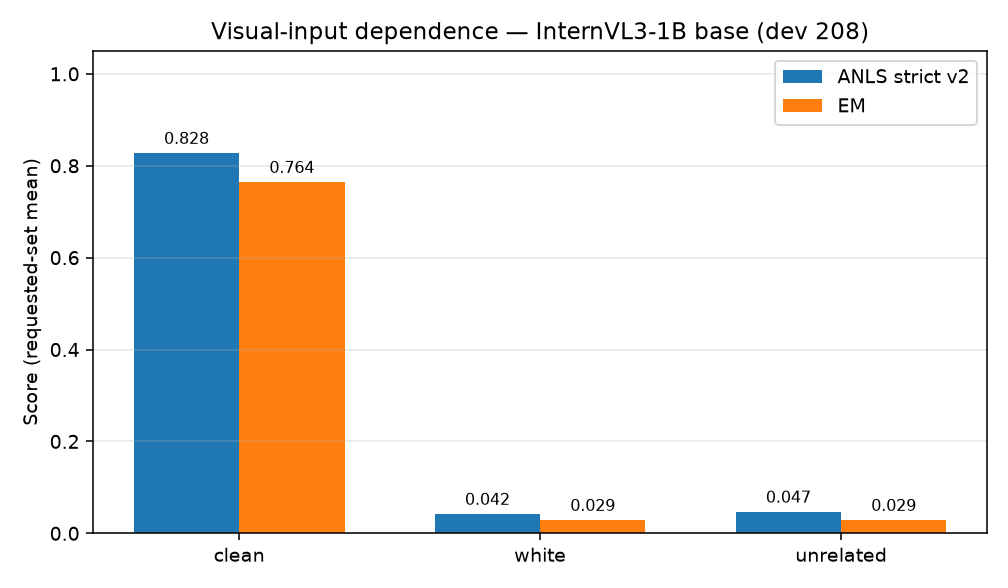
\includegraphics[width=0.78\linewidth]{visual_dependence_anls_em.png}
\caption{Visual-input dependence: requested-set ANLS and EM for clean, white, and unrelated conditions.}
\label{fig:visdep}
\end{figure}

\paragraph{Interpretation.}
Replacing the correct page with a white or unrelated image reduced development ANLS by approximately 78 percentage points, indicating strong dependence on the correct visual input.
Unrelated scores use the original question's references (mismatch diagnostic; layout/tiles may change).
White/clean tile histograms matched \emph{in this run} (observation, not a general law).
Residual correct answers do not establish memorization or contamination; the study does not prove fine-grained visual grounding.

\paragraph{Mapping deviation.}
Original protocol wording described ascending donor QID then residual seeded shuffle.
Executed code: among equal minimum aspect-distance donors, seeded choice via \texttt{random.Random(2026).choice} (candidates ordered by QID).
Frozen mapping retained; not regenerated.

\begin{figure}[H]
\centering
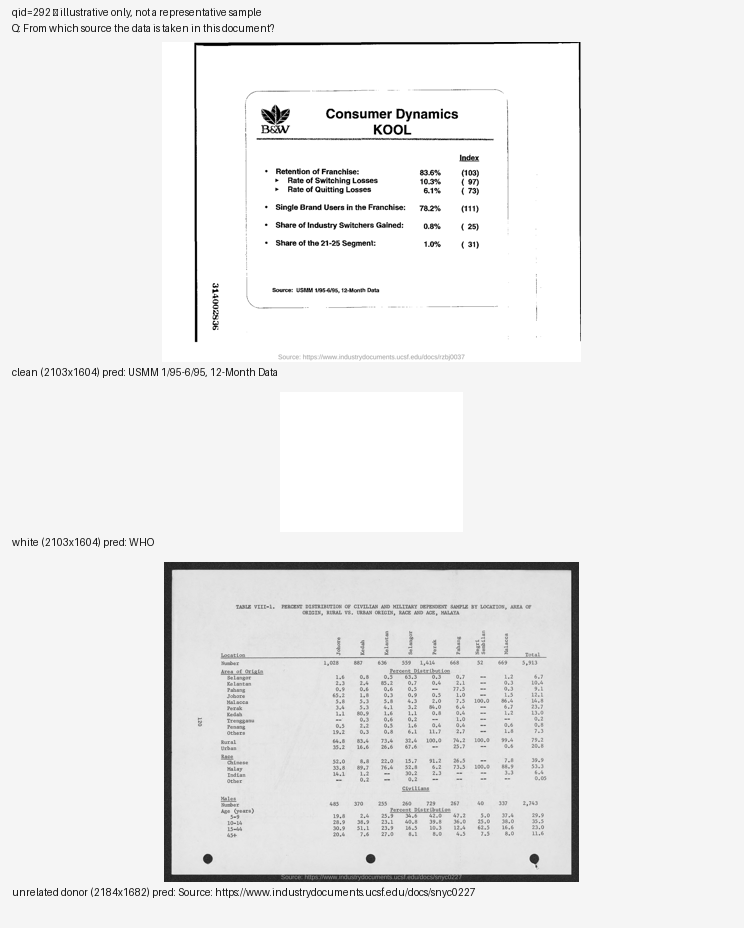
\includegraphics[width=0.88\linewidth]{gallery_00_qid_292.png}
\caption{Illustrative visual-dependence example (qid 292; stacked clean / white / unrelated). Deterministic selection: clean EM${=}1$, white EM${=}0$; not a representative sample.}
\label{fig:visgal}
\end{figure}

\begin{figure}[H]
\centering
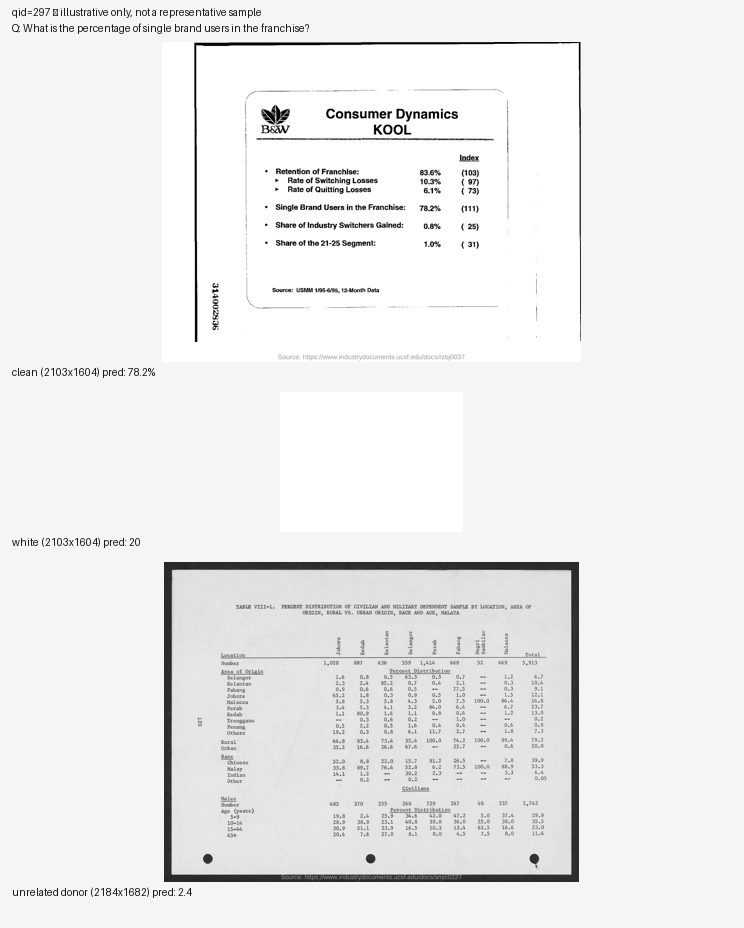
\includegraphics[width=0.88\linewidth]{gallery_01_qid_297.png}
\caption{Illustrative visual-dependence example (qid 297; same selection rule as Figure~\ref{fig:visgal}).}
\end{figure}

\begin{figure}[H]
\centering
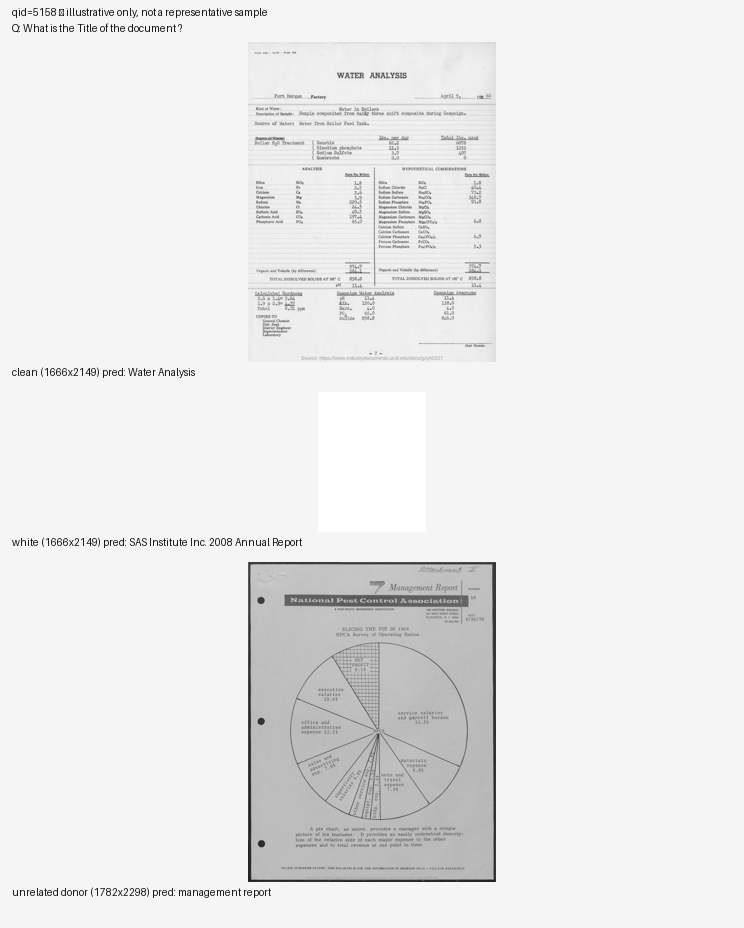
\includegraphics[width=0.88\linewidth]{gallery_02_qid_5158.png}
\caption{Illustrative visual-dependence example (qid 5158; same selection rule as Figure~\ref{fig:visgal}).}
\end{figure}

\begin{figure}[H]
\centering
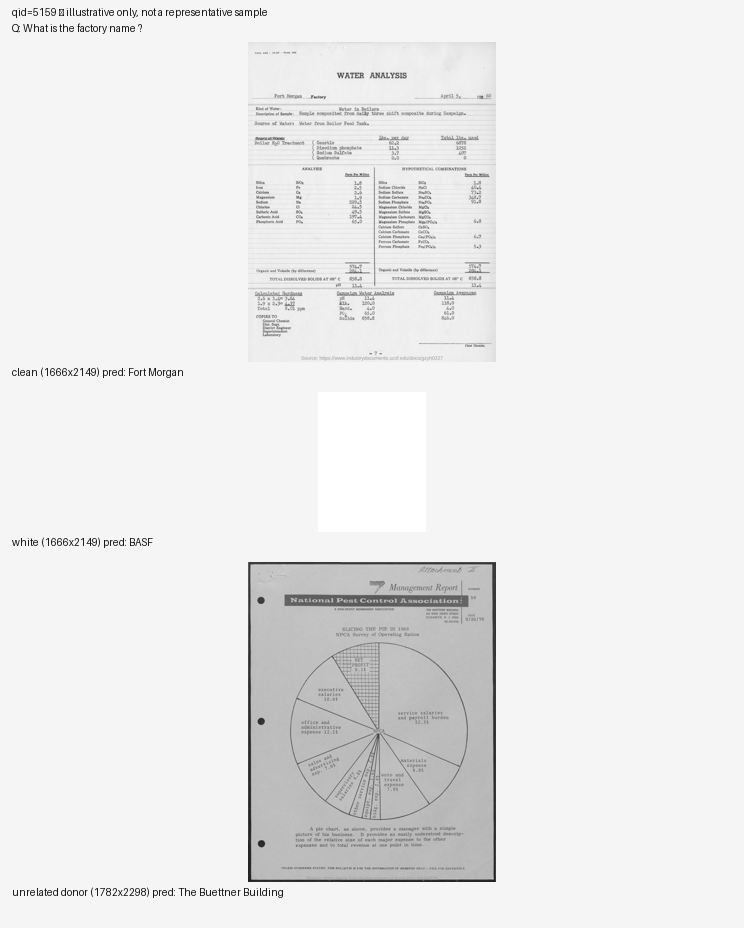
\includegraphics[width=0.88\linewidth]{gallery_03_qid_5159.png}
\caption{Illustrative visual-dependence example (qid 5159; same selection rule as Figure~\ref{fig:visgal}).}
\end{figure}

\paragraph{Reproduction pointers.}
Companion protocols: \texttt{docs/companion/pascal/}.
Compact tables/figures: \texttt{companion/pascal/results/}.
Primary inference/loading path remains the root project loader (\texttt{load\_internvl} + \texttt{load\_language\_lora}); PEFT \texttt{base\_model\_name\_or\_path} is stale inherited metadata (see \texttt{docs/report/adapter\_metadata\_audit.md}).

\bibliographystyle{plainnat}
\bibliography{references}

\end{document}
